\documentclass[a4paper]{article}
\usepackage{amsmath}
\usepackage{graphicx}
\usepackage{geometry}
\usepackage{floatrow}
\usepackage{layout}
\usepackage{amssymb} 
\usepackage{multirow}
\usepackage[utf8]{inputenc}
\usepackage{caption}
\geometry{margin=1in}
\usepackage{authblk}
\usepackage{indentfirst}
\usepackage{multicol}
%\usepackage{biblatex}
\usepackage{cite}
\begin{document}
\title{\textbf{\huge{ENS210 Group \#3 Project Report}}}
\author{\textbf\large{Berra Say{\i}n \vspace{3ex} Fatih Ta\c{s}yaran \vspace{3ex} Rana Kalkan} \\ \vspace{-4ex} \textit{Instructor: Ogün Adebali}}
%\affiliation{The	College,	University	of	Chicago,	Chicago,	Illinois	60637,	USA}
%\affil{\textbf{Sichuan University,	Chengdu,		China}}
\date{\today}
%	Abstract
\maketitle
%\begin{thebibliography}{10}
%\end{thebibliography}

\section{Introduction}

Characterizing a protein family in an evolutionary aspect could give hints about function, evolutionary history, critical residues and domains of this protein family. In order to observe a protein's functionality across animals which live in aquatic and terrestrial environments and also animals like tetrapods who live in intersection of this environments, we chose the protein family \textbf{Carbamoyl-phosphate synthase, large subunit (CPS)}.
\par
\smallskip
CPS catalyses the synthesis of carbamoyl phosphate from biocarbonate, ATP and glutamine  or ammonia and represents the first committed step in pyrimidine and arginine biosynthesis in prokaryotes and eukaryotes, and in the urea cycle in most terrestrial vertebrates.
Most prokaryotes carry one form of CPS that participates in both arginine and pyrimidine biosynthesis, however certain bacteria can have separate forms. Eukaryotes have two different forms of CPS: a mitochondrial enzyme (CPSI) that participates in both arginine biosynthesis and the urea cycle; and a cytosolic enzyme (CPSII) involved in pyrimidine biosynthesis.There is a third form of the enzyme, CPSIII, found in fish, which uses glutamine as a nitrogen source instead of ammonia.
\par
\smallskip
In general, animals who live in different environments have different excretory systems. However, animals who live in the same environment and who are different kind of species can also have different excretory system. By examining the protein family which is one of the families that differ within different excretory systems, we are aiming to find evolutionary history of this protein family and it's effect on the phenotypes of different species.
\par
\smallskip
Ammonia is poisonous to all vertebrate, although it is not dangerous in low density and a good solvent in water. Therefore, it is possible to excrete ammonia for animals who  live in abundance of water called aquatic animals. In contrary, there is no such feasibility for terrestrial animals so that they have to convert ammonia into urea or uric acid in their livers by reacting ammonia with $CO_2$ via the urea cycle and excrete urea with consuming more energy due to this process.
\par
\smallskip
As mentioned before, species and their excretory systems are intervening in terms of environments. Whales who are mammals excrete urea in contrary to marine fishes. But some fishes which live in very alkaline environments excrete urea in contrary to marine fishes. Also there is the case of animals like amphibians, which live in both of these two environments, demonstrates three of this nitrogen waste forms. Because of this variety, we want to investigate the evolutionary history of the protein family of \textbf{CPS} that has a significant role in this process. 

\section{Method}
To be able to investigate this evolutionary history, we acquired sequences of \textbf{CPSI}, \textbf{CPSII} and \textbf{CPSIII} via biological databases such as BLAST, PFAM, InterPro and GenBank for different species that have characteristics we mentioned above. To understand the homology between many species, we also looked at OrthoDB where we can find numerous orthologous sequences. Then, we aligned those sequences via MEGA and R using \textit{ClustalW} algorithm. In order to specifically observe mutated residues and conserved residues we permuted all 3 variants in a pairwise manner which are:

\begin{itemize}
\begin{multicols}{3}
    \item CPSI(1)
    \item CPSII(2)
    \item CPSIII(3)
    \columnbreak
    \item CPSI - CPSII(4)
    \item CPSI - CPSIII(5)
    \item CPSII - CPSIII(6)
    \columnbreak
    \item CPSI - CPSII- CPSIII(7)
    \item Consensusses of \\ CPSI, CPSII \& CPSIII(8)
    \end{multicols}
\end{itemize}

\begin{figure}[H]
\begin{center}
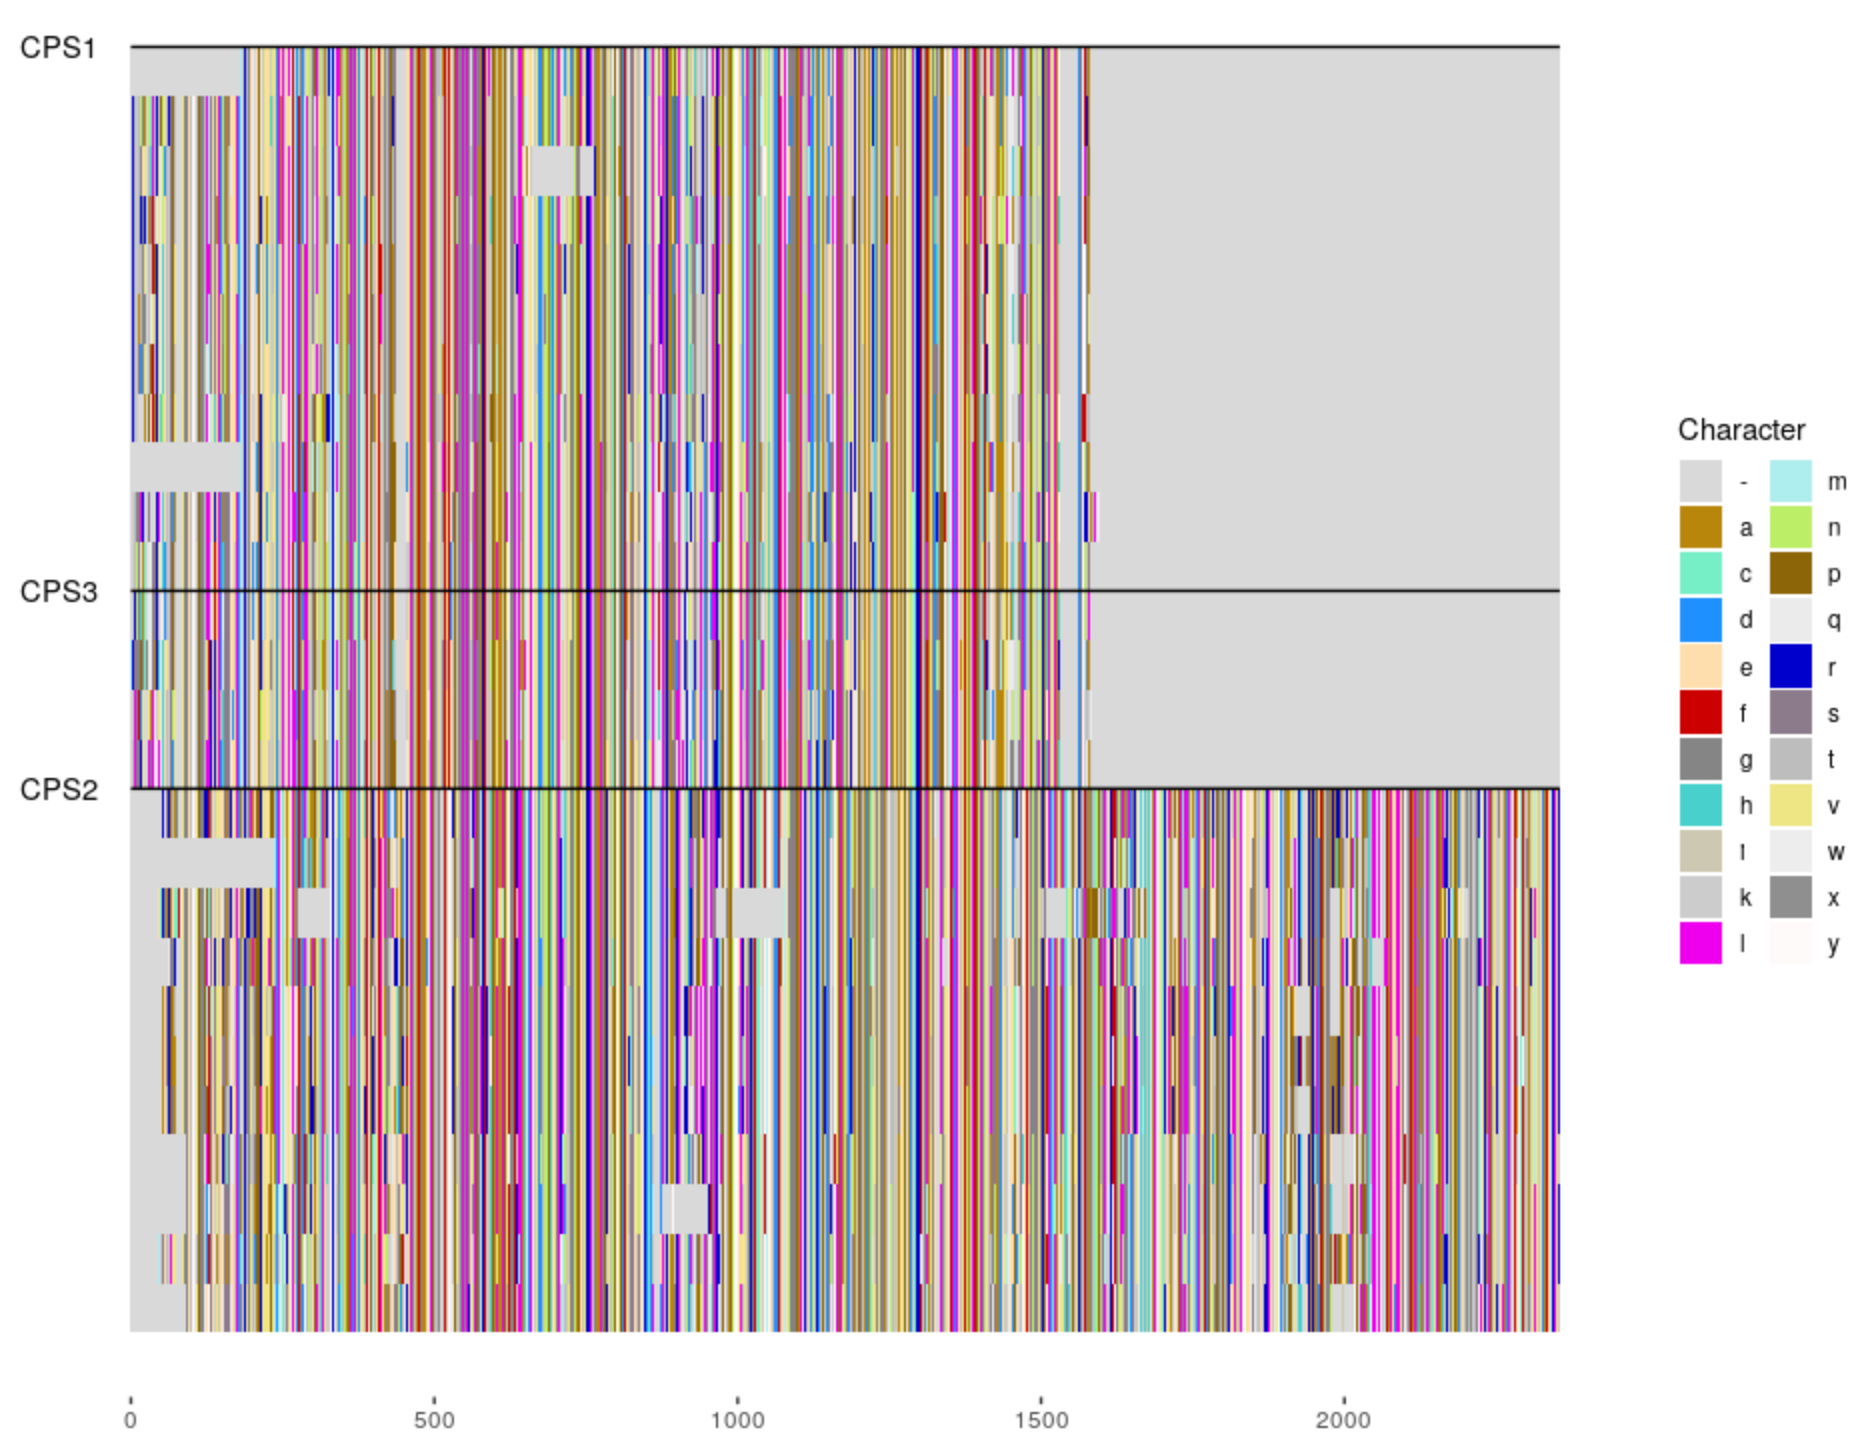
\includegraphics[width=\textwidth]{draw_aline.png}
\end{center}
\caption{Visual Interpretation of Multiple Sequence Alignments}
\label{fig:visual}
\end{figure}

We aligned mentioned $8$ combinations of sequences and we looked at their \textit{Heatmap of Distances}, \textit{Visual Interpretation}, \textit{Conserved Residue positions and it's overlapping over domains} and \textit{Pylogenetic Tree}. To find the critical positions, we also grouped the sources of this as sequences as \textit{Amniotes}, \textit{Amphibians} and \textit{Aquatics}.

\par
\smallskip
First we aligned protein sequences of a small samples (11 species from CPSI, 11 species from CPSII and 4 species from CPSIII) from distinct taxonomic groups in Jawed vertebrates which are Birds,Alligators and others, Turtles, Lizards, Mammals,Amphibians, Coelacanths, Bony Fishes, Cartilaginous fishes, Fig~\ref{fig:visual}. We observed that CPSII has longer sequence than CPSI and CPSIII which are almost has same length of sequence. 
Then we looked at their conserved residues Fig~\ref{fig:conserved}. 

\newpage

\begin{figure}[H]
\begin{center}
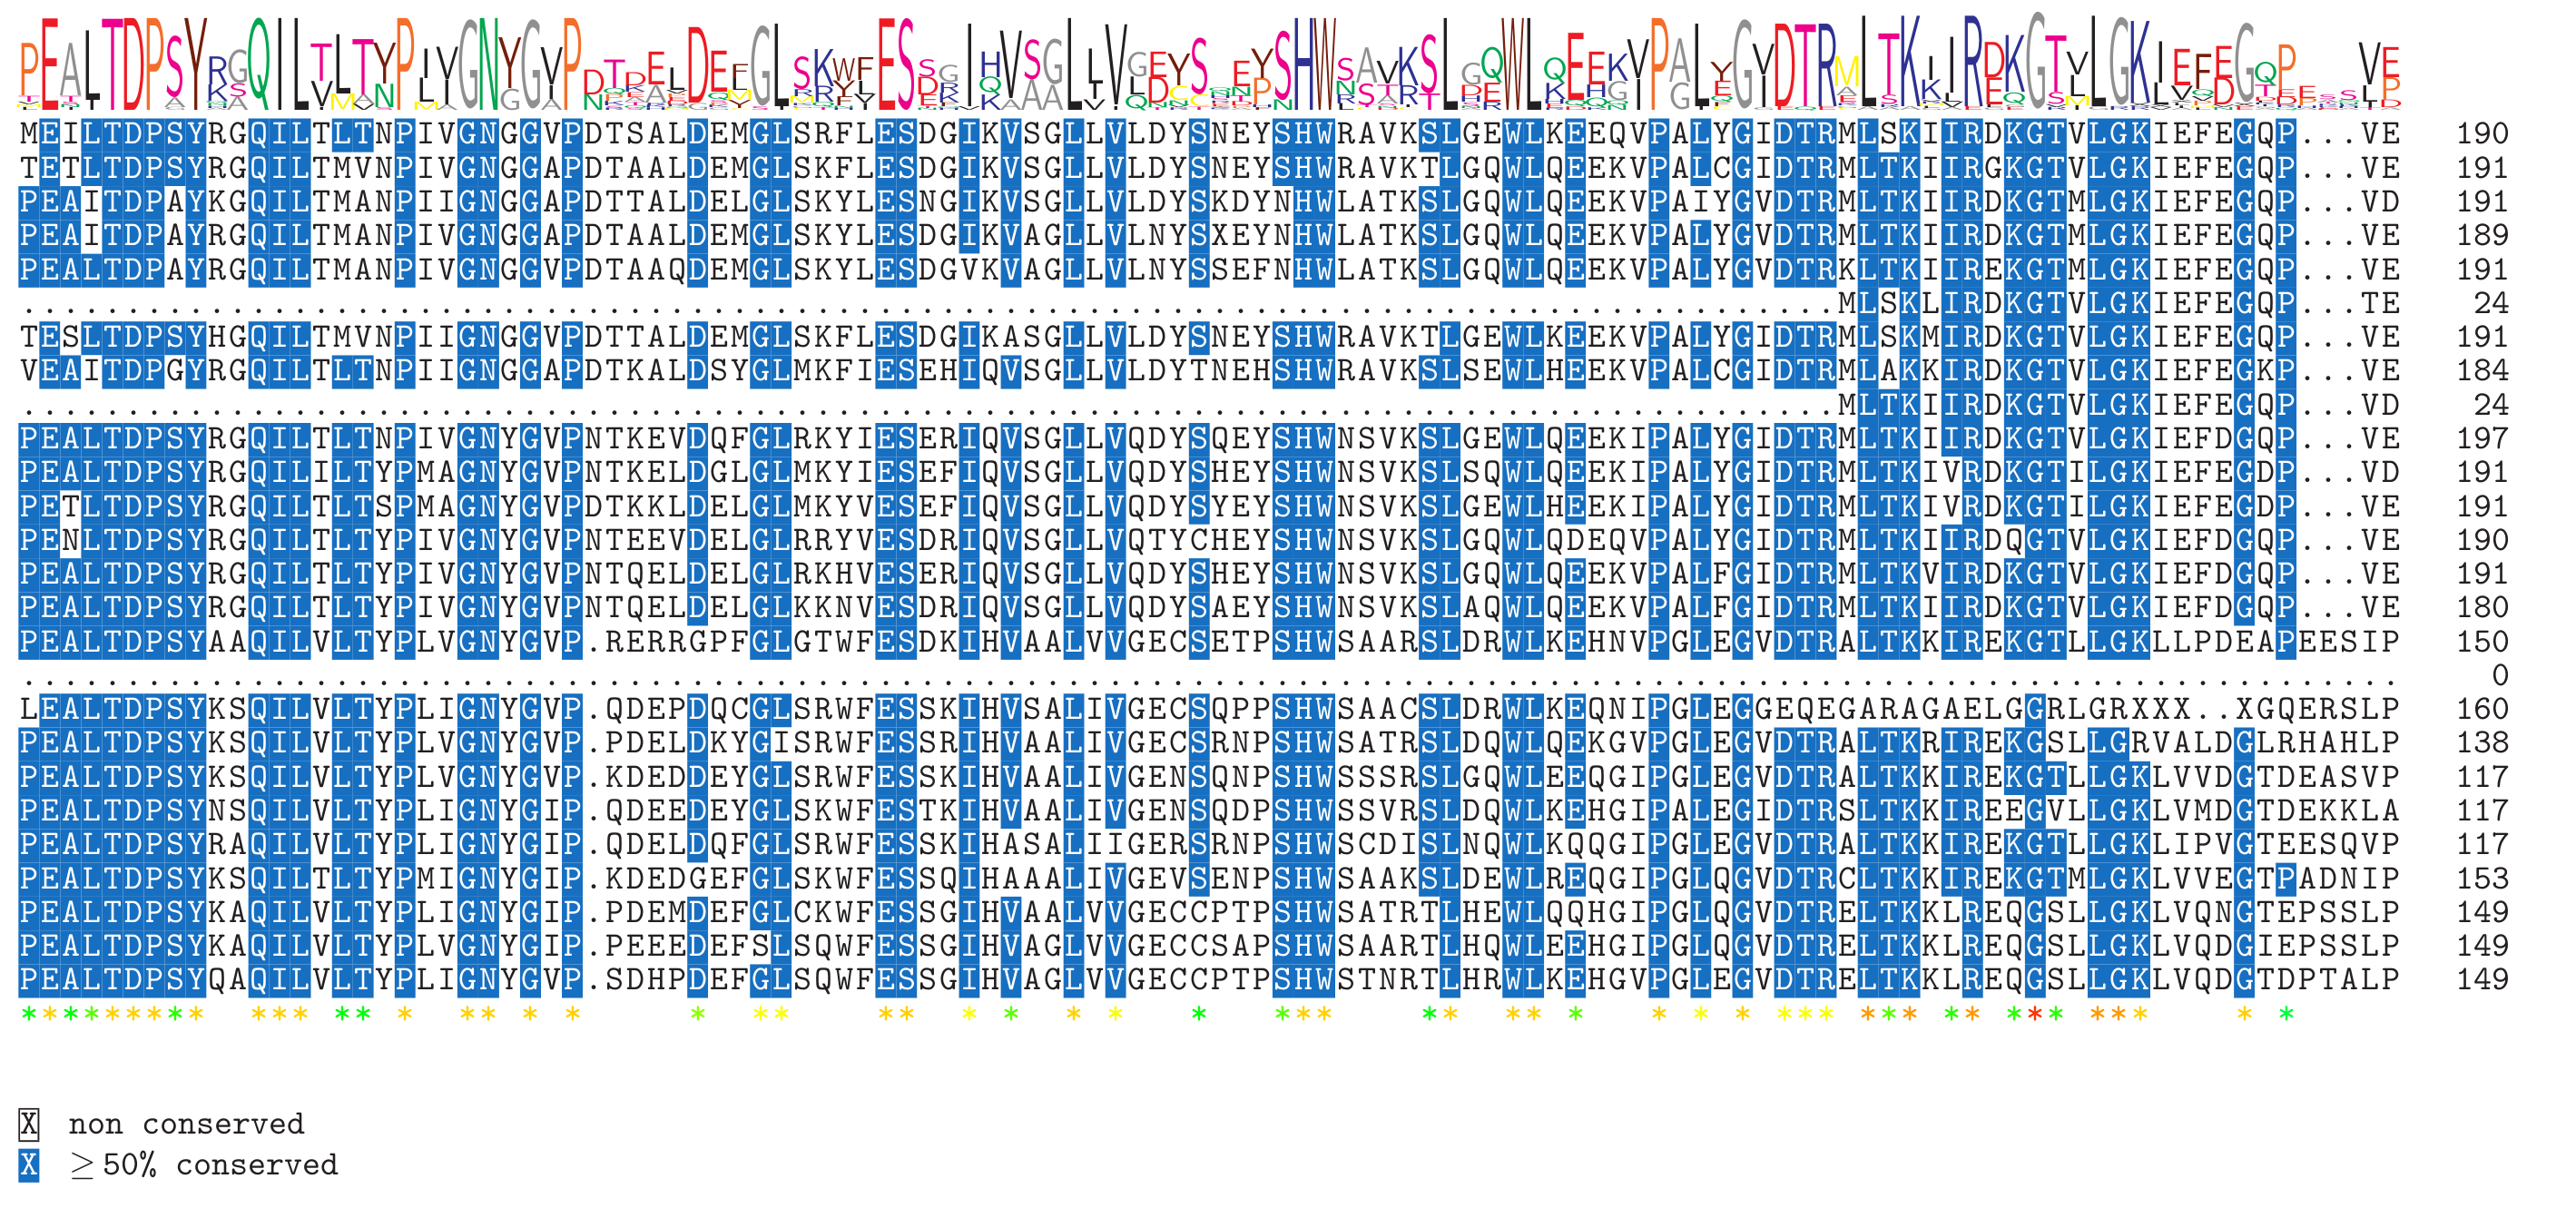
\includegraphics[width=\textwidth]{conserved.png}
\end{center}
\caption{Conserved Residues Among \textbf{CPSI-II-III}}
\label{fig:conserved}
\end{figure}

After calculating conserved residues and visual interpretations, we draw a heatmap of distance between aligned sequences for the species in the small subset to specifically see which of them closer to each other. In this interpretation we found out \textit{Human}, \textit{Platypus} and \textit{Koala} are closer to each other than other animals.Fig~\ref{fig:heatmap} We also observed this situation in phylogenetic tree we draw and also we observed relatedness among Rooster and Crocodile. Which increased our confidence level in our work since these two species are also closer in the evolutionary tree. Fig~\ref{fig:tree}

\begin{figure}[H]
\begin{center}
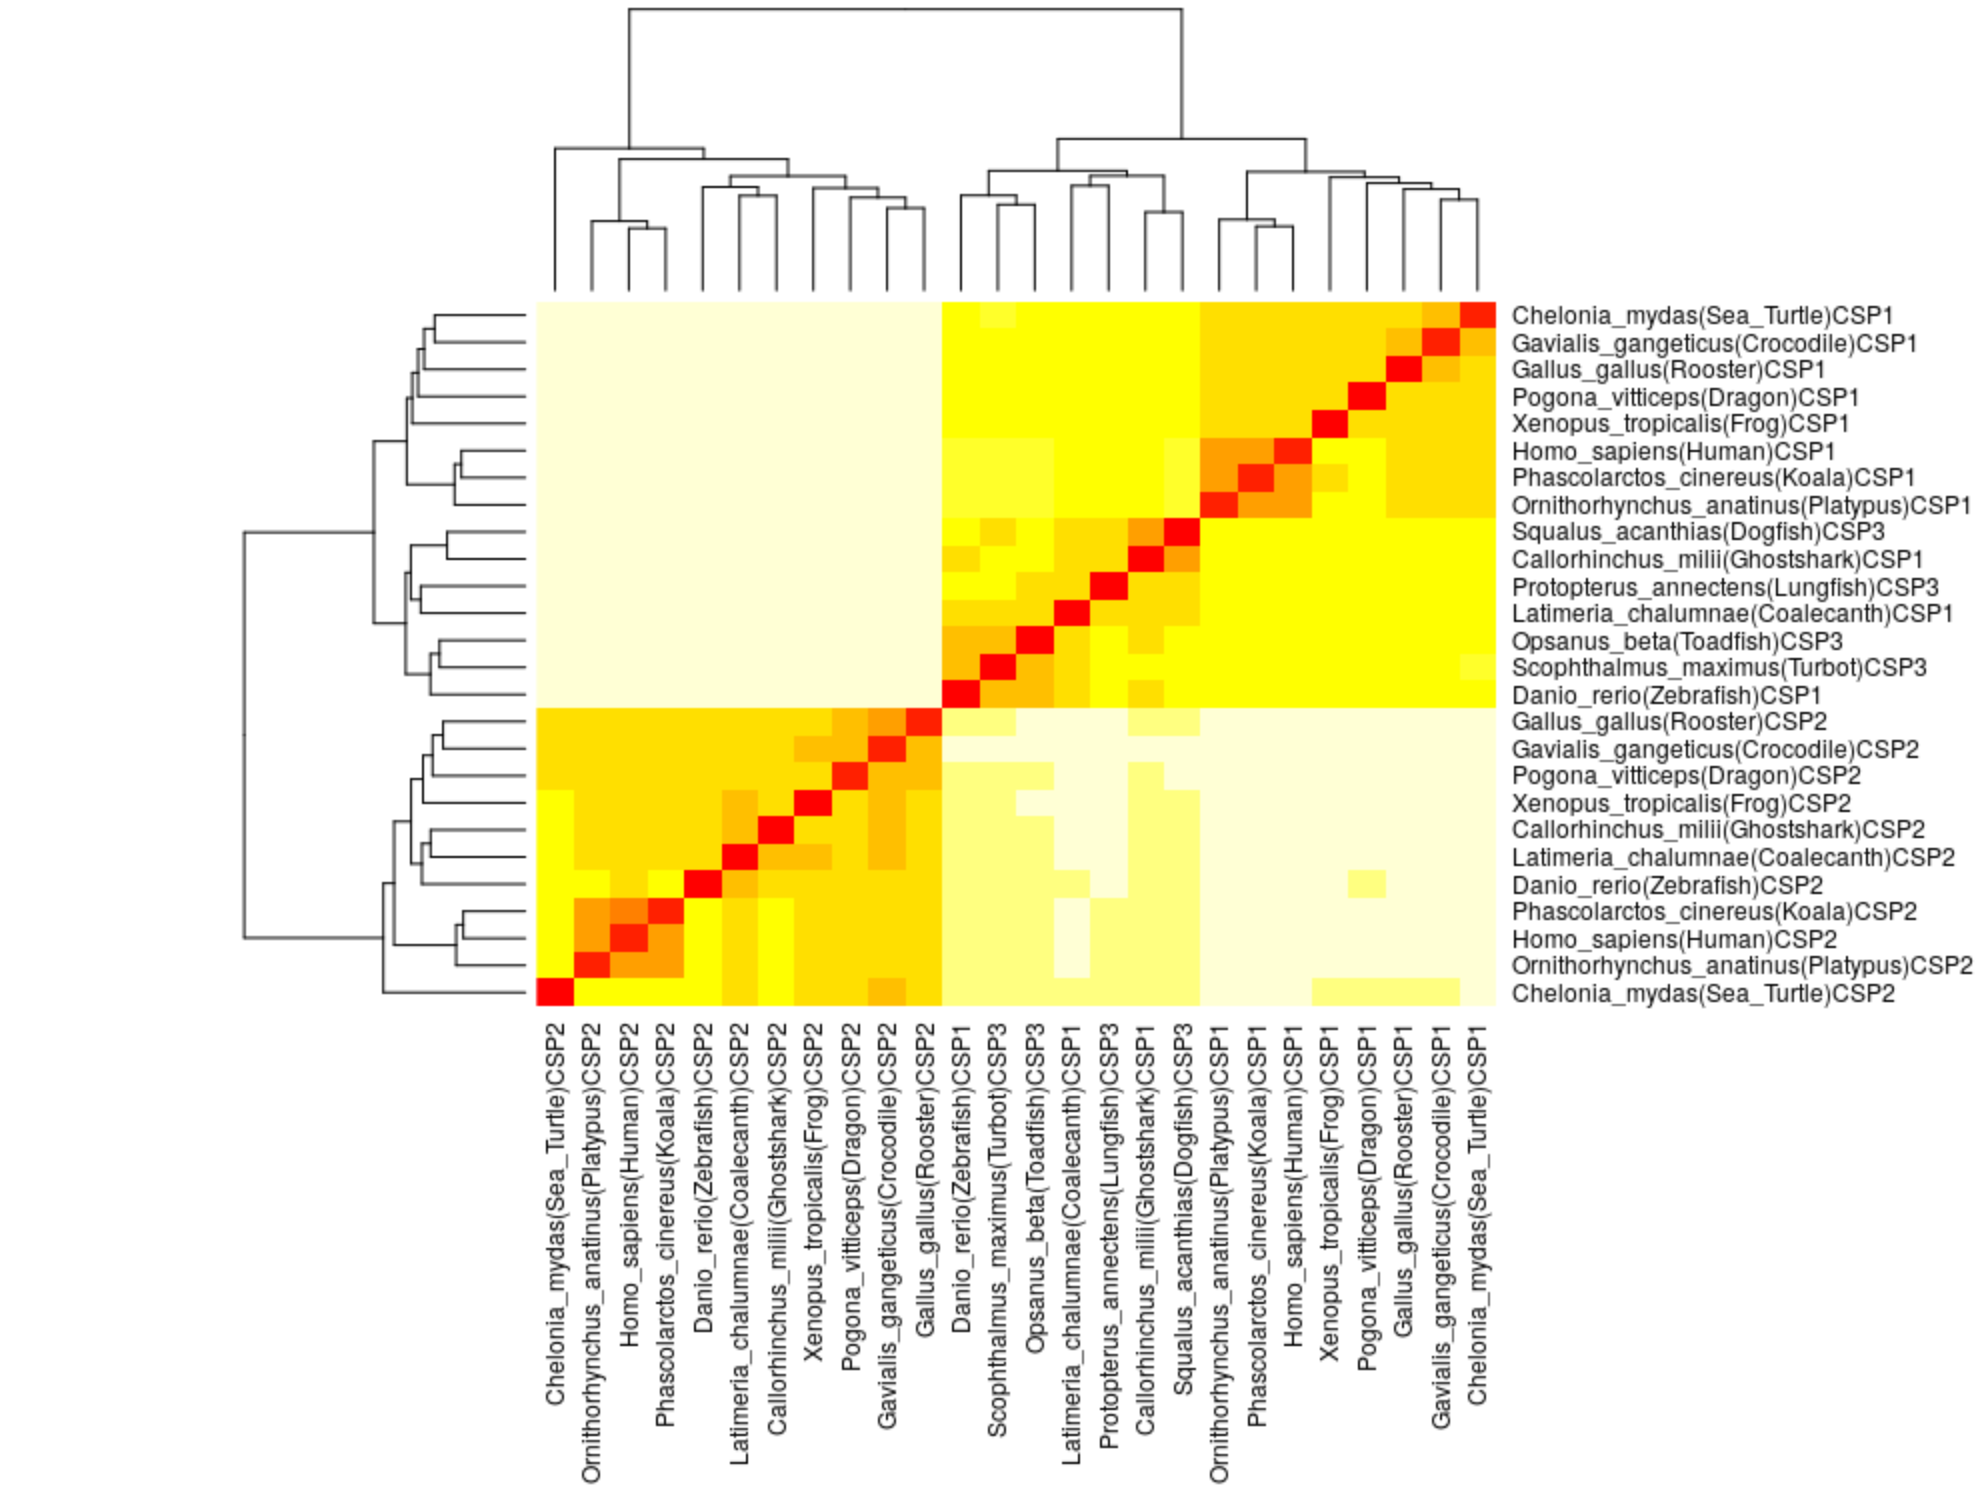
\includegraphics[width=.8\textwidth]{heatmap.png}
\end{center}
\caption{Heat map of Distances of Aligned Sequences Belong to Different Species}
\label{fig:heatmap}
\end{figure}

\newpage

\begin{figure}[H]
\begin{center}
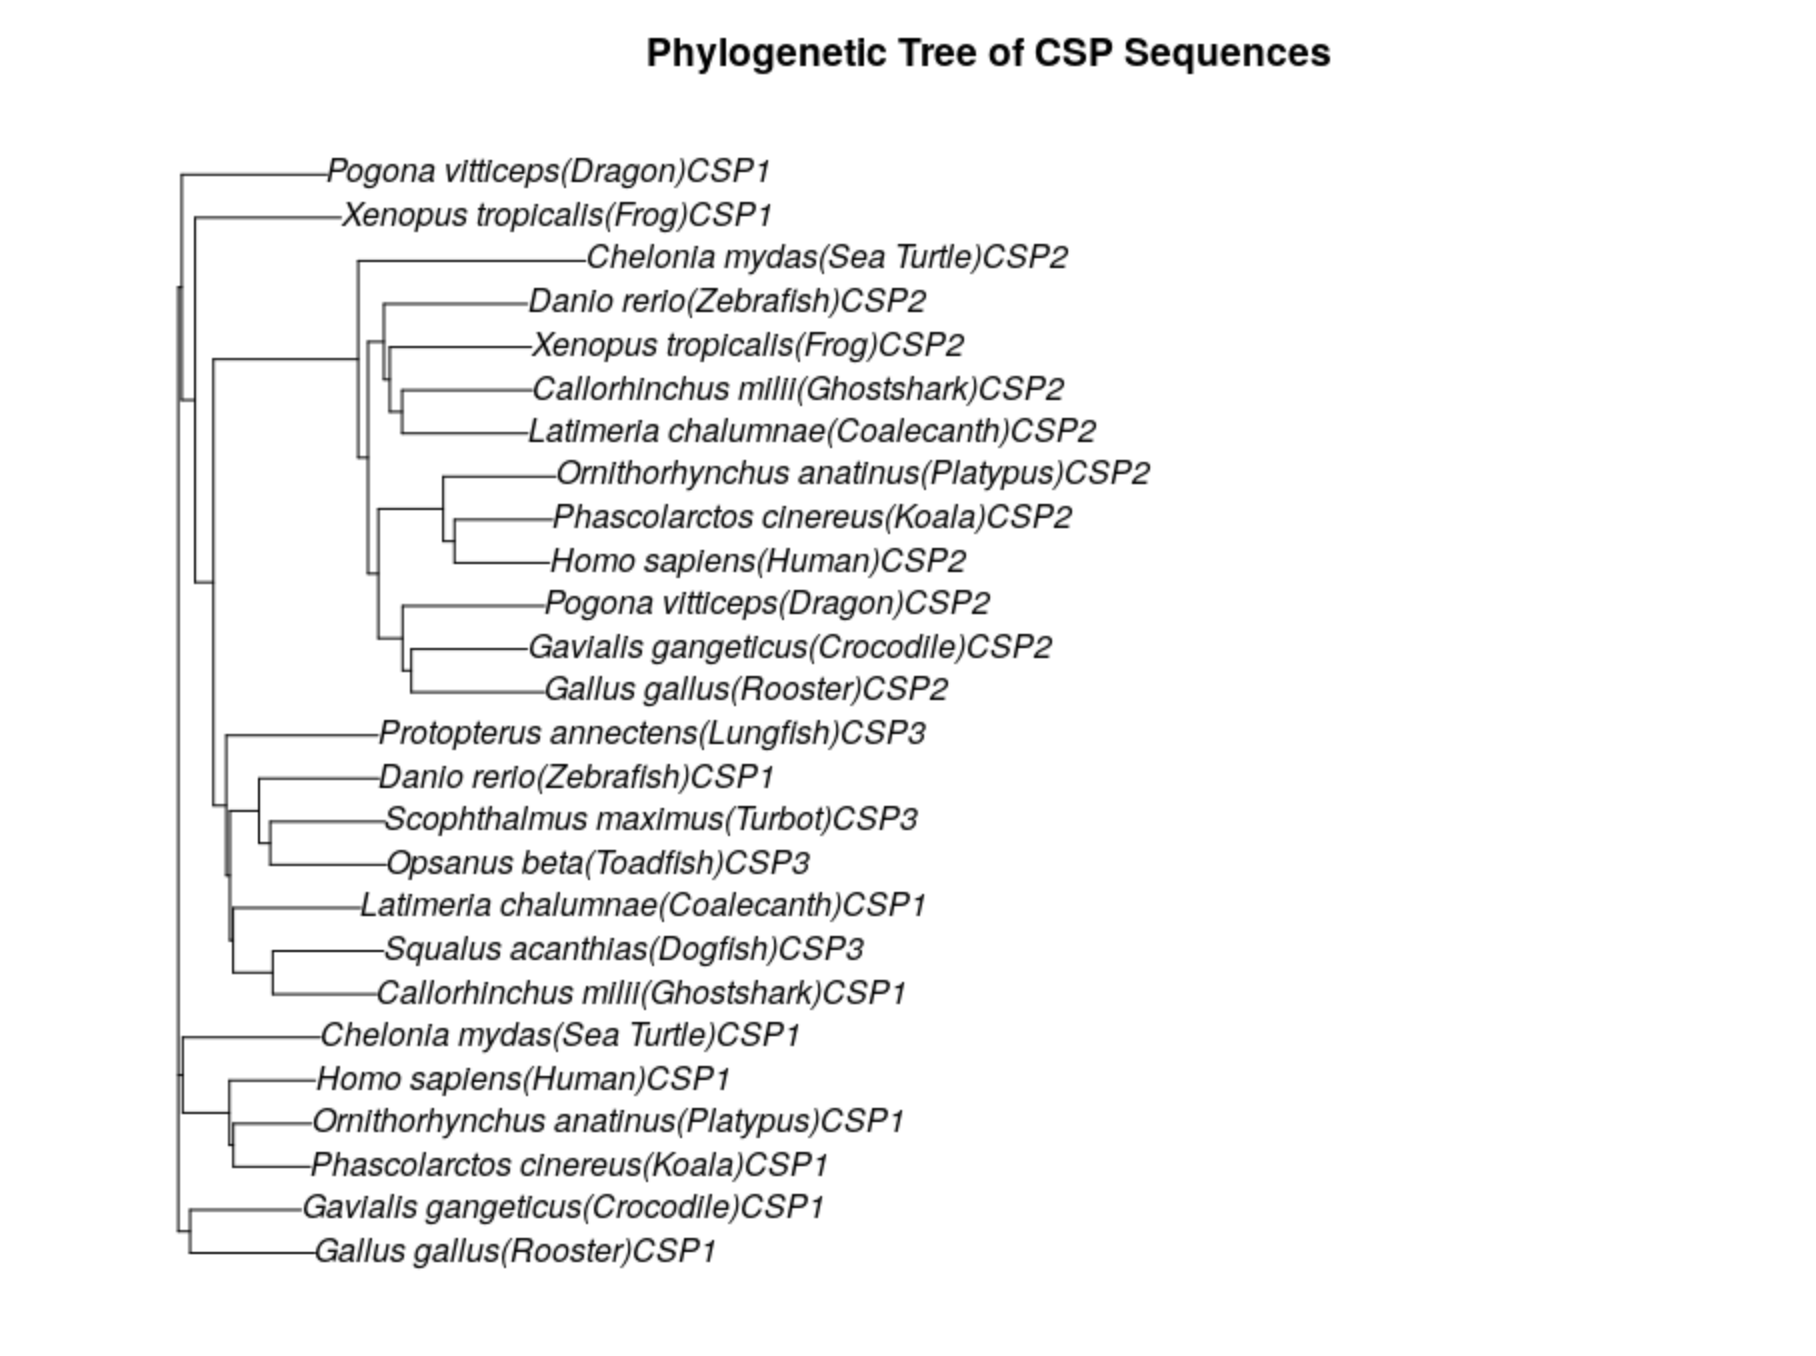
\includegraphics[width=\textwidth]{tree.png}
\end{center}
\caption{Phylogenetic Tree of Small Dataset}
\label{fig:tree}
\end{figure}
Then we expanded our samples and collected 10 protein sequences \cite{CPSI}\cite{CPSII}\cite{blast}\cite{interpro7-client}\cite{pfam} from each group of Jawed vertabrates as we mentioned. Then we had 110 sequences from CPSI and CPSII and 4 sequences from CPSIII since we found a few samples in databanks. After that we aligned them as a group of CPSI-CPSII, CPSI-CPSIII, CPSII-CPSIII and CPSI-CPSII-CPSIII. Then we calculated conservation scores for each alignments and plotted their graphs Fig~\ref{fig:biggraph1}. We also identified positions of protein domains and then added those regions belonging to distinct domains into our plots in different colors.\cite{conserved} We observed that CPSase-L-D2 domain which is represented in green region is less conserved compared to others. This domain is Carbamoyl-phosphate synthase L chain, ATP binding domain and it has an ATP-grasp fold.  

\newpage
\begin{figure}[H]
\begin{center}
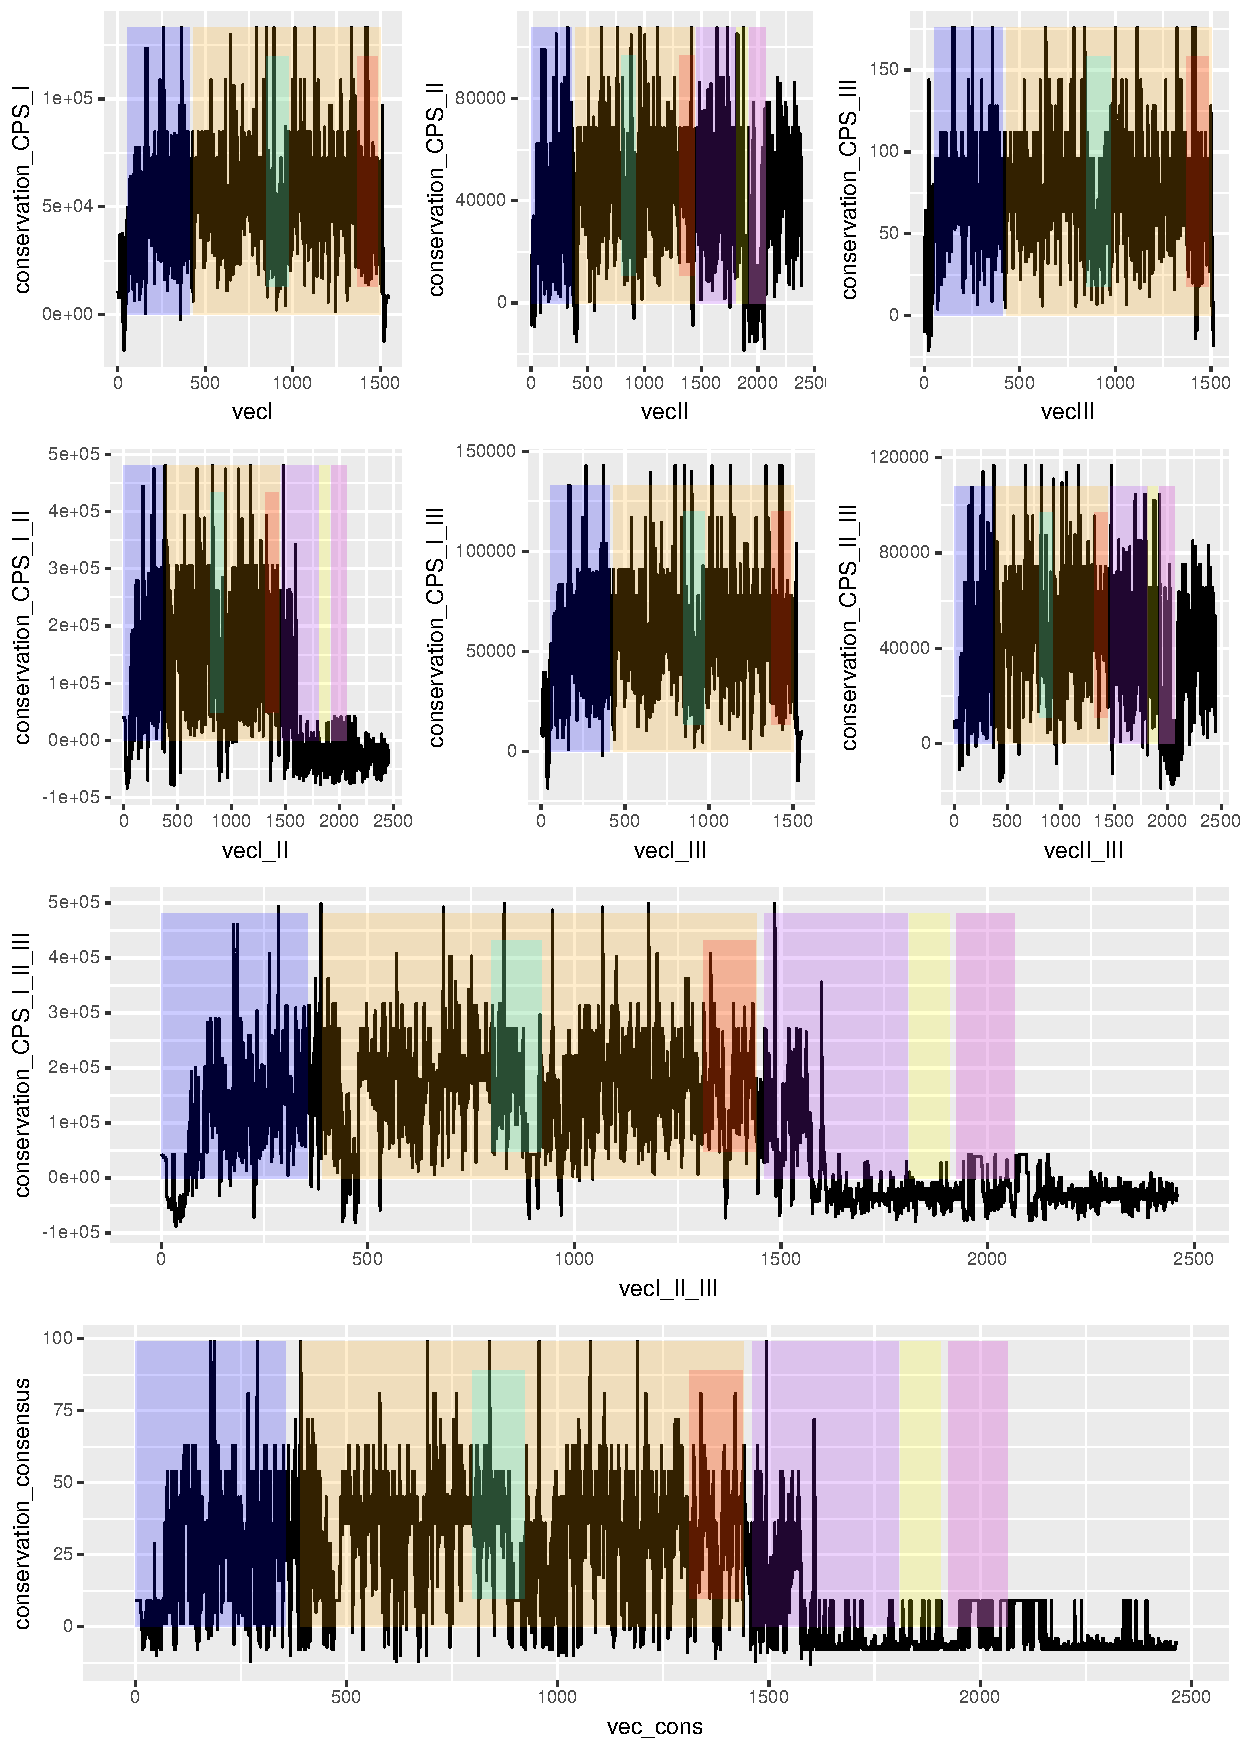
\includegraphics[width=\textwidth]{pairwise.pdf}
\end{center}
\caption{Conserved Residues Among \textbf{CPSI-II-III}}
\label{fig:biggraph1}
\end{figure}

\newpage

\newpage
\begin{figure}[H]
\begin{center}
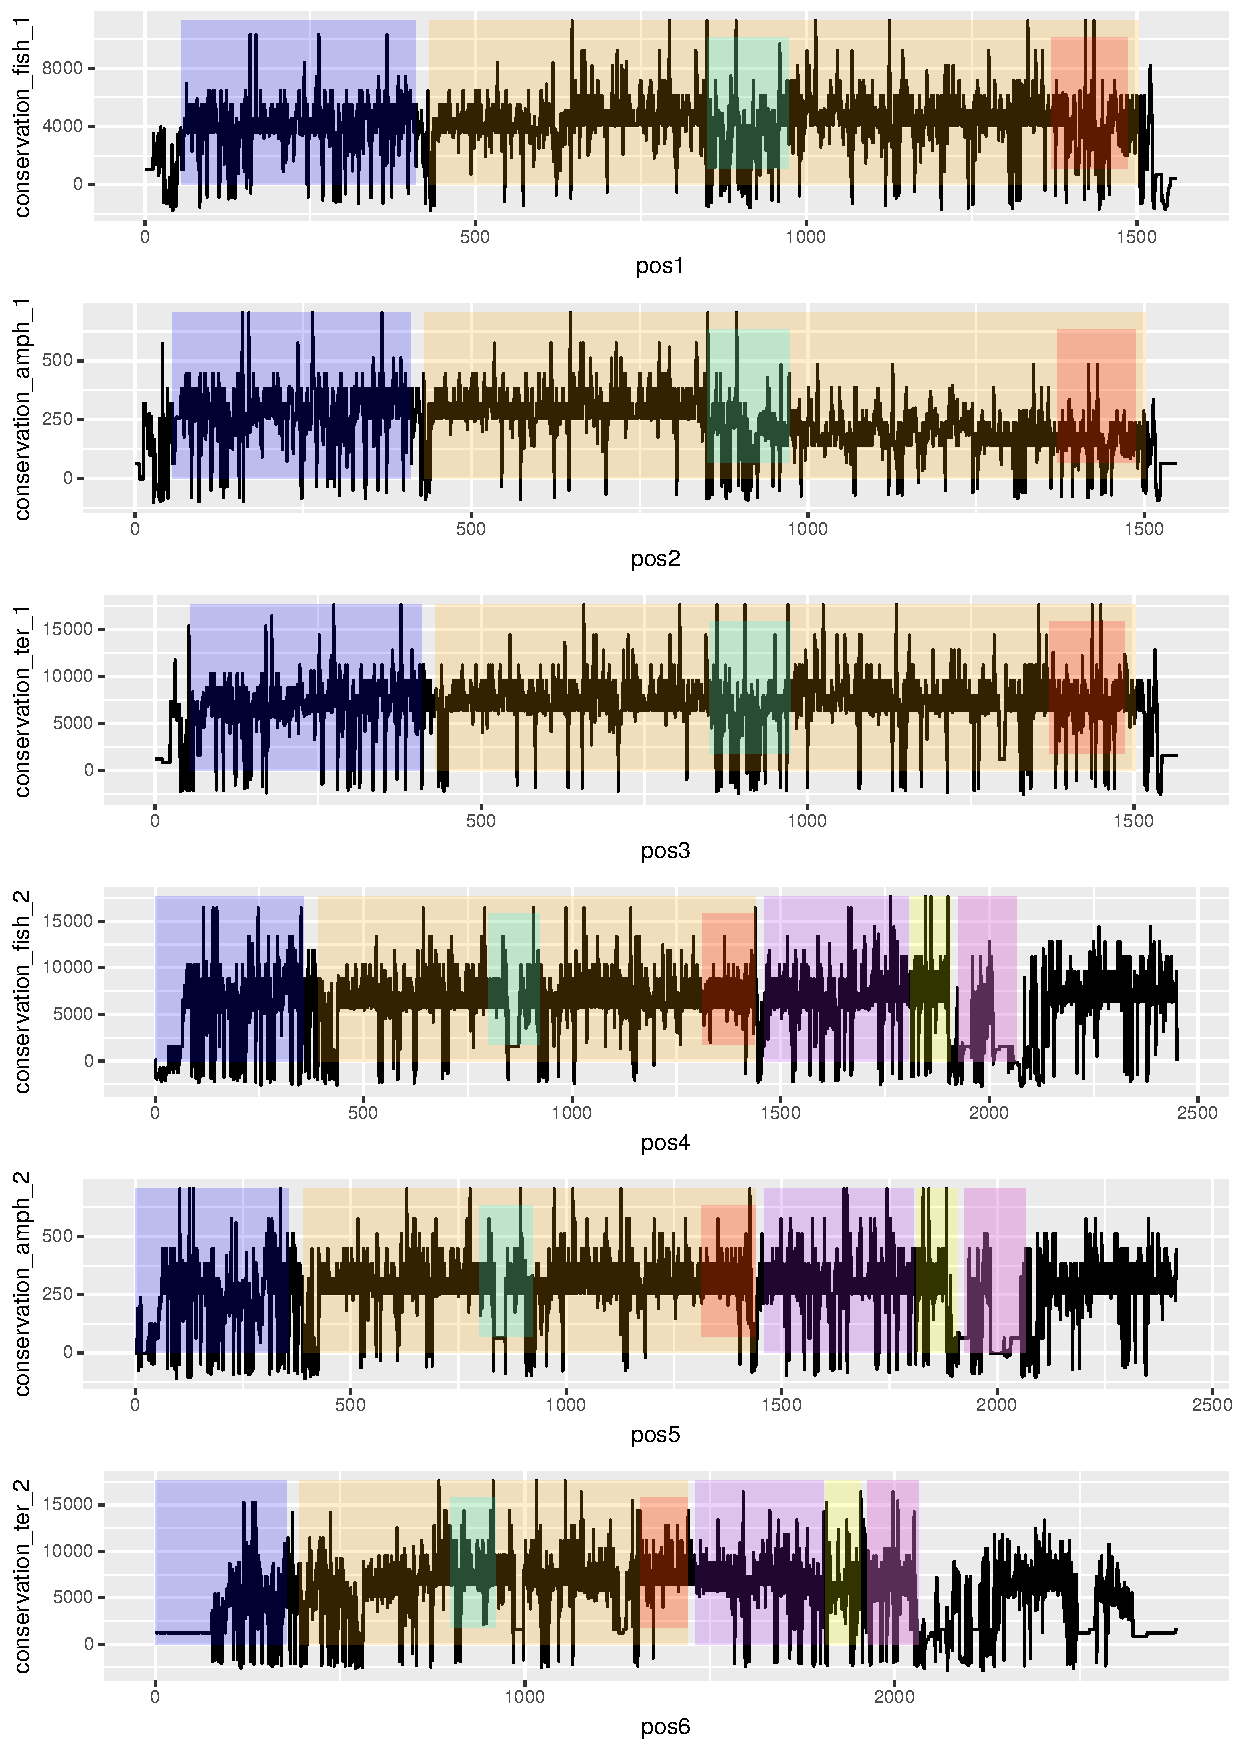
\includegraphics[width=\textwidth]{vsconsensus.pdf}
\end{center}
\caption{Conserved Residues \textbf{CPSI} belongs to (1)Fishes, (2)Amphibians, (3)Terrestrial Animals and \textbf{CPSII} belongs to (4)Fishes, (5)Amphibians, (6)Terrestrial Animal. Consensus among all \textbf{CPSI} and \textbf{CPSII} given equal weight for this comparison.}
\label{fig:biggraph2}
\end{figure}

\section{Results & Discussion}
Due to time limitations, we could not make all our calculations ready, but finally, we compared consensus for CPSI, CPSII and CPSIII to sequences acquired from different species (fish, amphibian and terrestrial). Results are given in Fig~\ref{fig:biggraph2}. We observed some domains are related to big variations among species while some domains are strictly conserved.

%To illustrate, terrestrial animals excrete urea since they libe in an environment which don't have abundance of water and 

\bibliography{references}{}
\bibliographystyle{plain}


\end{document}